\section{Requirements}

\begin{figure}[t]
  \begin{center}
  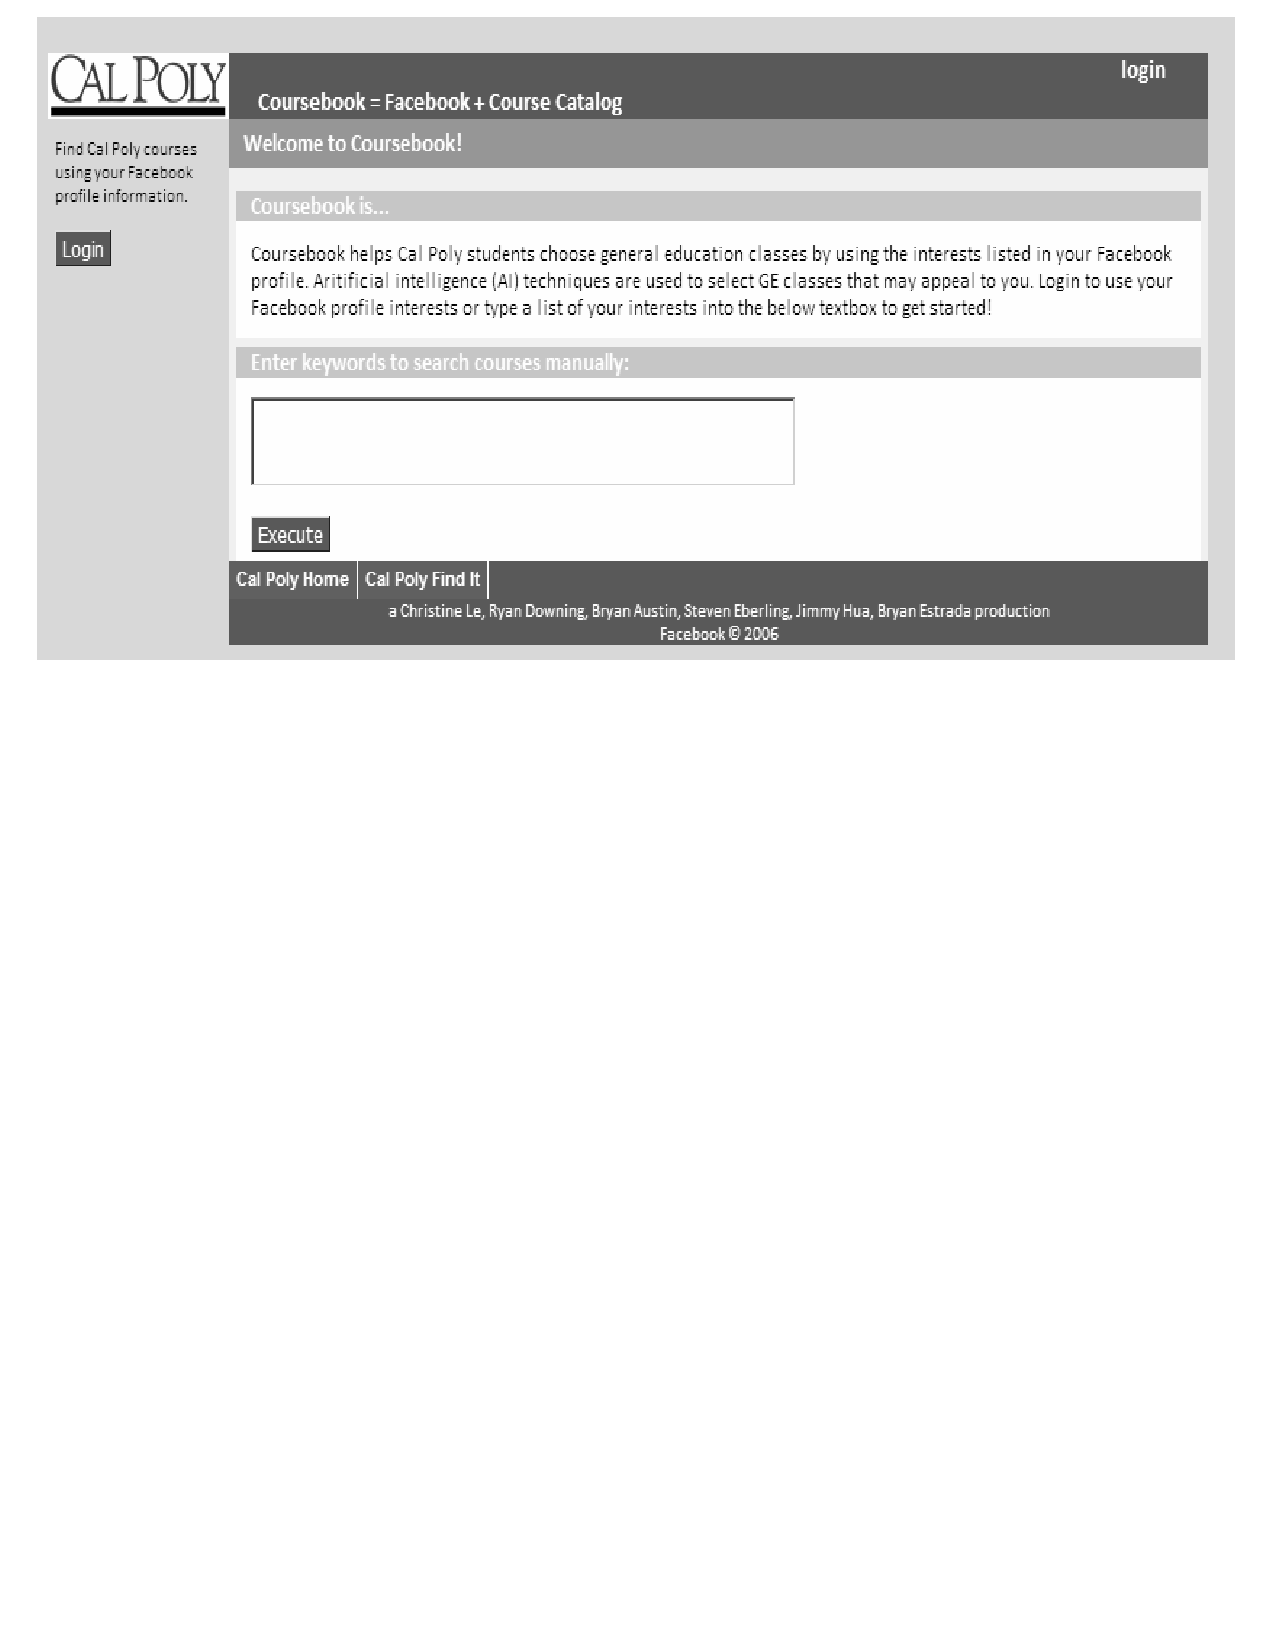
\includegraphics[scale=0.75]{images/screenshot}
  \caption{Coursebook Screenshot}
  \label{fig:screenshot}
  \end{center}
\end{figure}

\subsubsection*{Web User Interface}
By implementing Coursebook with a web-based user interface, we present users 
with an easily accessible service. Coursebook utilizes the latest technologies 
on the J2EE stack, including the Spring framework, JDBC, and WordNet APIs to 
produce a highly responsive system that is platform agnostic on both the server
side (Java) and client side (DHTML/Javascript).

\subsubsection*{Live Data}
Coursebook consists of multiple distributed components to provide users with 
information. The system relies on a MySQL database for real-time course catalog
information. The Facebook API provides developers access to its users' profile 
information. Coursebook offers multiple points of entry, including automatic 
Facebook connectivity and manual user input, in case the former system is 
inaccessible.

\subsubsection*{Relevant Courses}
Coursebook uses advanced artificial intelligence techniques to search and 
compute the most applicable courses for each individual user.

\section{Distributed Components}
\begin{figure}[t]
  \begin{center}
  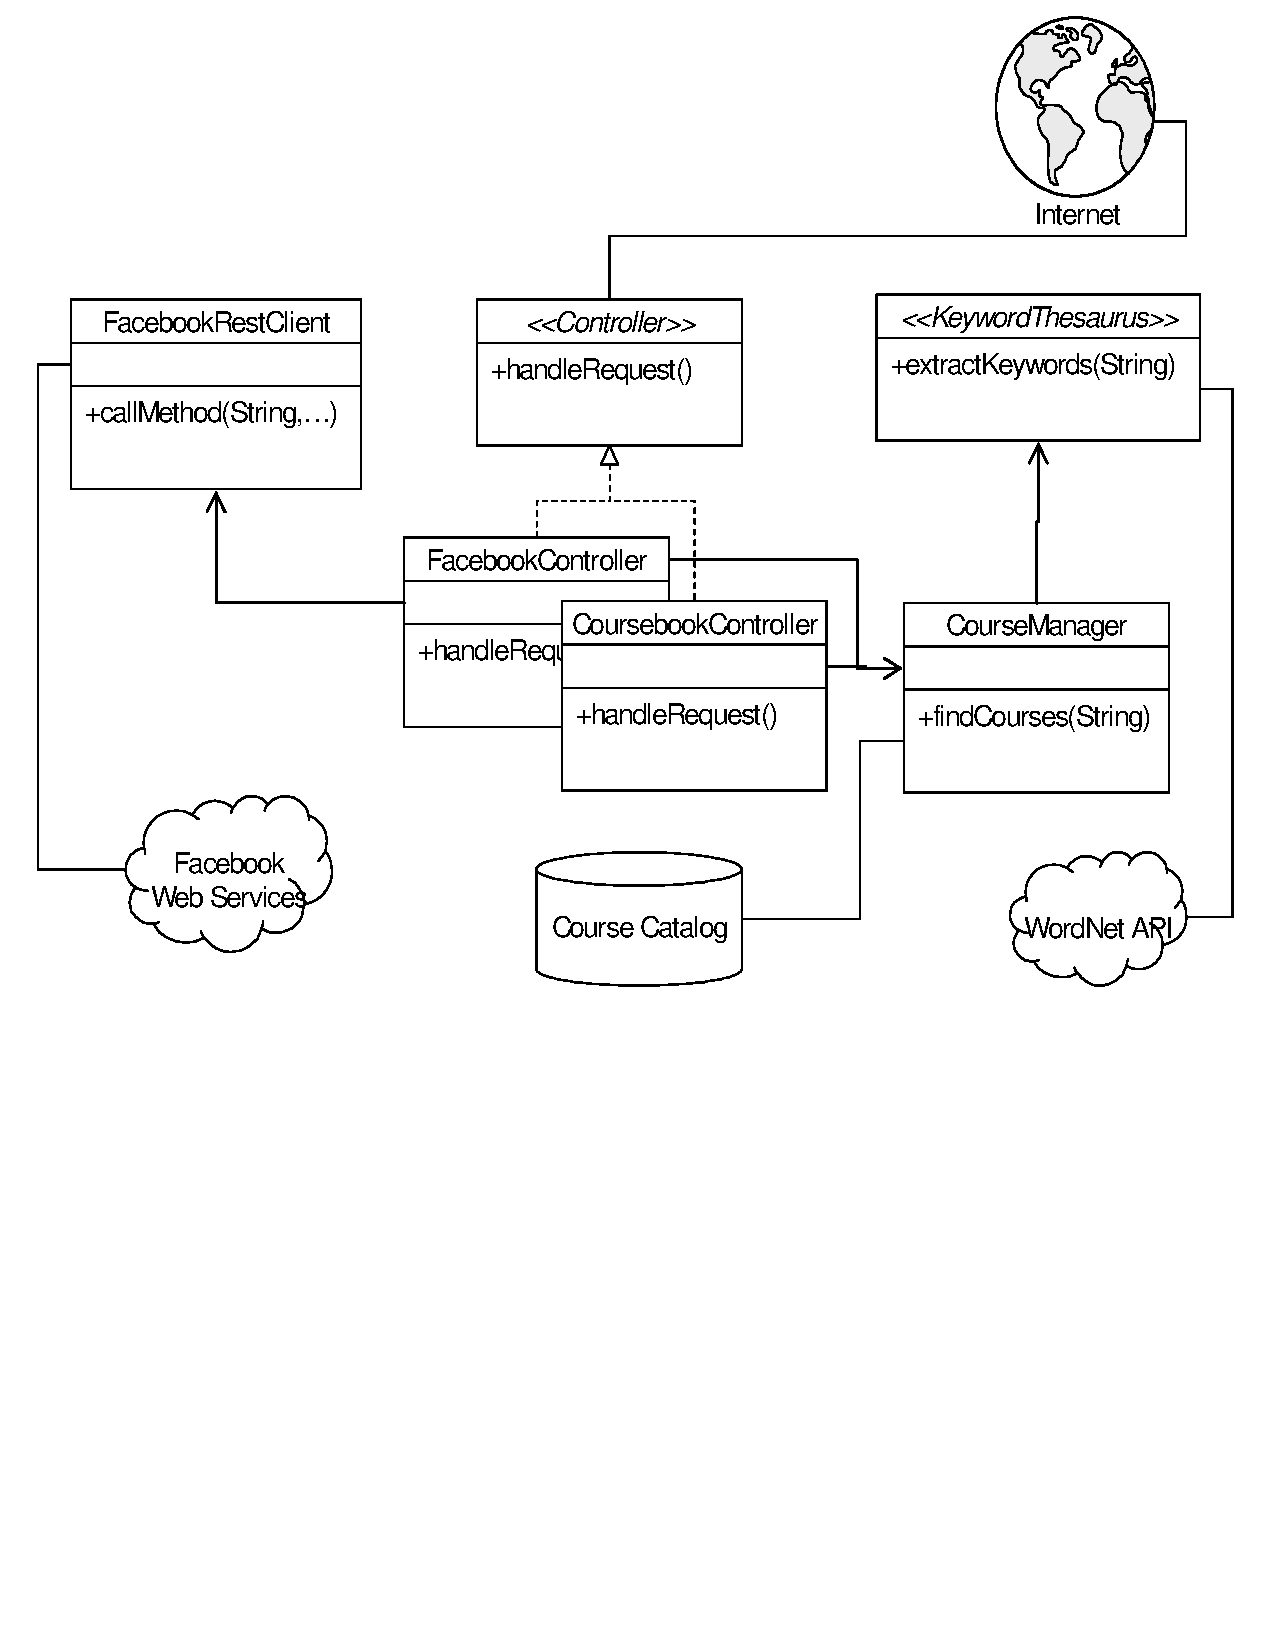
\includegraphics[width=\textwidth]{images/classes}
  \caption{Coursebook Abridged Class Diagram}
  \label{fig:classes}
  \end{center}
\end{figure}

